% Options for packages loaded elsewhere
% Options for packages loaded elsewhere
\PassOptionsToPackage{unicode}{hyperref}
\PassOptionsToPackage{hyphens}{url}
\PassOptionsToPackage{dvipsnames,svgnames,x11names}{xcolor}
%
\documentclass[
  spanish,
  11pt,
  a4paper,
  DIV=11,
  numbers=noendperiod]{scrartcl}
\usepackage{xcolor}
\usepackage[margin=2.5cm]{geometry}
\usepackage{amsmath,amssymb}
\setcounter{secnumdepth}{5}
\usepackage{iftex}
\ifPDFTeX
  \usepackage[T1]{fontenc}
  \usepackage[utf8]{inputenc}
  \usepackage{textcomp} % provide euro and other symbols
\else % if luatex or xetex
  \usepackage{unicode-math} % this also loads fontspec
  \defaultfontfeatures{Scale=MatchLowercase}
  \defaultfontfeatures[\rmfamily]{Ligatures=TeX,Scale=1}
\fi
\usepackage{lmodern}
\ifPDFTeX\else
  % xetex/luatex font selection
  \setmainfont[]{Times New Roman}
\fi
% Use upquote if available, for straight quotes in verbatim environments
\IfFileExists{upquote.sty}{\usepackage{upquote}}{}
\IfFileExists{microtype.sty}{% use microtype if available
  \usepackage[]{microtype}
  \UseMicrotypeSet[protrusion]{basicmath} % disable protrusion for tt fonts
}{}
\makeatletter
\@ifundefined{KOMAClassName}{% if non-KOMA class
  \IfFileExists{parskip.sty}{%
    \usepackage{parskip}
  }{% else
    \setlength{\parindent}{0pt}
    \setlength{\parskip}{6pt plus 2pt minus 1pt}}
}{% if KOMA class
  \KOMAoptions{parskip=half}}
\makeatother
% Make \paragraph and \subparagraph free-standing
\makeatletter
\ifx\paragraph\undefined\else
  \let\oldparagraph\paragraph
  \renewcommand{\paragraph}{
    \@ifstar
      \xxxParagraphStar
      \xxxParagraphNoStar
  }
  \newcommand{\xxxParagraphStar}[1]{\oldparagraph*{#1}\mbox{}}
  \newcommand{\xxxParagraphNoStar}[1]{\oldparagraph{#1}\mbox{}}
\fi
\ifx\subparagraph\undefined\else
  \let\oldsubparagraph\subparagraph
  \renewcommand{\subparagraph}{
    \@ifstar
      \xxxSubParagraphStar
      \xxxSubParagraphNoStar
  }
  \newcommand{\xxxSubParagraphStar}[1]{\oldsubparagraph*{#1}\mbox{}}
  \newcommand{\xxxSubParagraphNoStar}[1]{\oldsubparagraph{#1}\mbox{}}
\fi
\makeatother

\usepackage{color}
\usepackage{fancyvrb}
\newcommand{\VerbBar}{|}
\newcommand{\VERB}{\Verb[commandchars=\\\{\}]}
\DefineVerbatimEnvironment{Highlighting}{Verbatim}{commandchars=\\\{\}}
% Add ',fontsize=\small' for more characters per line
\usepackage{framed}
\definecolor{shadecolor}{RGB}{241,243,245}
\newenvironment{Shaded}{\begin{snugshade}}{\end{snugshade}}
\newcommand{\AlertTok}[1]{\textcolor[rgb]{0.68,0.00,0.00}{#1}}
\newcommand{\AnnotationTok}[1]{\textcolor[rgb]{0.37,0.37,0.37}{#1}}
\newcommand{\AttributeTok}[1]{\textcolor[rgb]{0.40,0.45,0.13}{#1}}
\newcommand{\BaseNTok}[1]{\textcolor[rgb]{0.68,0.00,0.00}{#1}}
\newcommand{\BuiltInTok}[1]{\textcolor[rgb]{0.00,0.23,0.31}{#1}}
\newcommand{\CharTok}[1]{\textcolor[rgb]{0.13,0.47,0.30}{#1}}
\newcommand{\CommentTok}[1]{\textcolor[rgb]{0.37,0.37,0.37}{#1}}
\newcommand{\CommentVarTok}[1]{\textcolor[rgb]{0.37,0.37,0.37}{\textit{#1}}}
\newcommand{\ConstantTok}[1]{\textcolor[rgb]{0.56,0.35,0.01}{#1}}
\newcommand{\ControlFlowTok}[1]{\textcolor[rgb]{0.00,0.23,0.31}{\textbf{#1}}}
\newcommand{\DataTypeTok}[1]{\textcolor[rgb]{0.68,0.00,0.00}{#1}}
\newcommand{\DecValTok}[1]{\textcolor[rgb]{0.68,0.00,0.00}{#1}}
\newcommand{\DocumentationTok}[1]{\textcolor[rgb]{0.37,0.37,0.37}{\textit{#1}}}
\newcommand{\ErrorTok}[1]{\textcolor[rgb]{0.68,0.00,0.00}{#1}}
\newcommand{\ExtensionTok}[1]{\textcolor[rgb]{0.00,0.23,0.31}{#1}}
\newcommand{\FloatTok}[1]{\textcolor[rgb]{0.68,0.00,0.00}{#1}}
\newcommand{\FunctionTok}[1]{\textcolor[rgb]{0.28,0.35,0.67}{#1}}
\newcommand{\ImportTok}[1]{\textcolor[rgb]{0.00,0.46,0.62}{#1}}
\newcommand{\InformationTok}[1]{\textcolor[rgb]{0.37,0.37,0.37}{#1}}
\newcommand{\KeywordTok}[1]{\textcolor[rgb]{0.00,0.23,0.31}{\textbf{#1}}}
\newcommand{\NormalTok}[1]{\textcolor[rgb]{0.00,0.23,0.31}{#1}}
\newcommand{\OperatorTok}[1]{\textcolor[rgb]{0.37,0.37,0.37}{#1}}
\newcommand{\OtherTok}[1]{\textcolor[rgb]{0.00,0.23,0.31}{#1}}
\newcommand{\PreprocessorTok}[1]{\textcolor[rgb]{0.68,0.00,0.00}{#1}}
\newcommand{\RegionMarkerTok}[1]{\textcolor[rgb]{0.00,0.23,0.31}{#1}}
\newcommand{\SpecialCharTok}[1]{\textcolor[rgb]{0.37,0.37,0.37}{#1}}
\newcommand{\SpecialStringTok}[1]{\textcolor[rgb]{0.13,0.47,0.30}{#1}}
\newcommand{\StringTok}[1]{\textcolor[rgb]{0.13,0.47,0.30}{#1}}
\newcommand{\VariableTok}[1]{\textcolor[rgb]{0.07,0.07,0.07}{#1}}
\newcommand{\VerbatimStringTok}[1]{\textcolor[rgb]{0.13,0.47,0.30}{#1}}
\newcommand{\WarningTok}[1]{\textcolor[rgb]{0.37,0.37,0.37}{\textit{#1}}}

\usepackage{longtable,booktabs,array}
\usepackage{calc} % for calculating minipage widths
% Correct order of tables after \paragraph or \subparagraph
\usepackage{etoolbox}
\makeatletter
\patchcmd\longtable{\par}{\if@noskipsec\mbox{}\fi\par}{}{}
\makeatother
% Allow footnotes in longtable head/foot
\IfFileExists{footnotehyper.sty}{\usepackage{footnotehyper}}{\usepackage{footnote}}
\makesavenoteenv{longtable}
\usepackage{graphicx}
\makeatletter
\newsavebox\pandoc@box
\newcommand*\pandocbounded[1]{% scales image to fit in text height/width
  \sbox\pandoc@box{#1}%
  \Gscale@div\@tempa{\textheight}{\dimexpr\ht\pandoc@box+\dp\pandoc@box\relax}%
  \Gscale@div\@tempb{\linewidth}{\wd\pandoc@box}%
  \ifdim\@tempb\p@<\@tempa\p@\let\@tempa\@tempb\fi% select the smaller of both
  \ifdim\@tempa\p@<\p@\scalebox{\@tempa}{\usebox\pandoc@box}%
  \else\usebox{\pandoc@box}%
  \fi%
}
% Set default figure placement to htbp
\def\fps@figure{htbp}
\makeatother



\ifLuaTeX
\usepackage[bidi=basic]{babel}
\else
\usepackage[bidi=default]{babel}
\fi
\ifPDFTeX
\else
\babelfont{rm}[]{Times New Roman}
\fi
% get rid of language-specific shorthands (see #6817):
\let\LanguageShortHands\languageshorthands
\def\languageshorthands#1{}


\setlength{\emergencystretch}{3em} % prevent overfull lines

\providecommand{\tightlist}{%
  \setlength{\itemsep}{0pt}\setlength{\parskip}{0pt}}



 


\usepackage{booktabs}
\usepackage{longtable}
\usepackage{array}
\usepackage{multirow}
\usepackage{wrapfig}
\usepackage{float}
\usepackage{colortbl}
\usepackage{pdflscape}
\usepackage{tabu}
\usepackage{threeparttable}
\usepackage{threeparttablex}
\usepackage[normalem]{ulem}
\usepackage{makecell}
\usepackage{xcolor}
\KOMAoption{captions}{tableheading}
\makeatletter
\@ifpackageloaded{caption}{}{\usepackage{caption}}
\AtBeginDocument{%
\ifdefined\contentsname
  \renewcommand*\contentsname{Tabla de contenidos}
\else
  \newcommand\contentsname{Tabla de contenidos}
\fi
\ifdefined\listfigurename
  \renewcommand*\listfigurename{Listado de Figuras}
\else
  \newcommand\listfigurename{Listado de Figuras}
\fi
\ifdefined\listtablename
  \renewcommand*\listtablename{Listado de Tablas}
\else
  \newcommand\listtablename{Listado de Tablas}
\fi
\ifdefined\figurename
  \renewcommand*\figurename{Figura}
\else
  \newcommand\figurename{Figura}
\fi
\ifdefined\tablename
  \renewcommand*\tablename{Tabla}
\else
  \newcommand\tablename{Tabla}
\fi
}
\@ifpackageloaded{float}{}{\usepackage{float}}
\floatstyle{ruled}
\@ifundefined{c@chapter}{\newfloat{codelisting}{h}{lop}}{\newfloat{codelisting}{h}{lop}[chapter]}
\floatname{codelisting}{Listado}
\newcommand*\listoflistings{\listof{codelisting}{Listado de Listados}}
\makeatother
\makeatletter
\makeatother
\makeatletter
\@ifpackageloaded{caption}{}{\usepackage{caption}}
\@ifpackageloaded{subcaption}{}{\usepackage{subcaption}}
\makeatother
\usepackage{bookmark}
\IfFileExists{xurl.sty}{\usepackage{xurl}}{} % add URL line breaks if available
\urlstyle{same}
\hypersetup{
  pdftitle={Análisis exploratorios},
  pdfauthor={Santos G},
  pdflang={es},
  colorlinks=true,
  linkcolor={blue},
  filecolor={Maroon},
  citecolor={Blue},
  urlcolor={Blue},
  pdfcreator={LaTeX via pandoc}}


\title{Análisis exploratorios}
\author{Santos G}
\date{}
\begin{document}
\maketitle

\renewcommand*\contentsname{Tabla de contenidos}
{
\hypersetup{linkcolor=}
\setcounter{tocdepth}{2}
\tableofcontents
}

\begin{Shaded}
\begin{Highlighting}[numbers=left,,]
\CommentTok{\# Librerías }
\FunctionTok{library}\NormalTok{(tidyverse)   }\CommentTok{\# Manipulación de datos: dplyr, tidyr, readr}
\FunctionTok{library}\NormalTok{(janitor)     }\CommentTok{\# Limpieza: clean\_names(), tabyl()}
\FunctionTok{library}\NormalTok{(ggplot2)     }\CommentTok{\# Gráficos profesionales}
\FunctionTok{library}\NormalTok{(skimr)       }\CommentTok{\# EDA rápido y completo (skim())}
\FunctionTok{library}\NormalTok{(GGally)      }\CommentTok{\# Matriz de gráficos para variables múltiples}
\FunctionTok{library}\NormalTok{(car)         }\CommentTok{\# Homocedasticidad (Levene)}
\FunctionTok{library}\NormalTok{(MVN)         }\CommentTok{\# Normalidad multivariada }
\FunctionTok{library}\NormalTok{(robustbase)  }\CommentTok{\# Detección de outliers}
\FunctionTok{library}\NormalTok{(knitr)       }\CommentTok{\# Tablas en Quarto}
\FunctionTok{library}\NormalTok{(kableExtra)  }\CommentTok{\# Tablas formateadas para informes}
\end{Highlighting}
\end{Shaded}

\section{Contexto general del
proyecto}\label{contexto-general-del-proyecto}

El presente proyecto corresponde a un análisis exploratorio de datos
morfométricos de tres especies del género \emph{Iris} (\emph{Iris
setosa}, \emph{Iris versicolor} e \emph{Iris virginica}). Este conjunto
de datos, ampliamente utilizado en estadística y aprendizaje automático,
contiene mediciones de longitud y anchura de sépalos y pétalos en un
total de 150 individuos (50 por especie).

El objetivo principal del análisis es describir y comparar la variación
morfológica entre especies, evaluando qué rasgos vegetativos (sépalos) y
reproductivos (pétalos) permiten una mejor discriminación taxonómica.

El trabajo se estructura en tres ejes:

\begin{enumerate}
\def\labelenumi{\arabic{enumi}.}
\tightlist
\item
  \textbf{Análisis descriptivo univariado y multivariado}: resumen
  numérico, visualizaciones (diagramas de dispersión, histogramas,
  gráficos de caja) y medidas de correlación.\\
\item
  \textbf{Evaluación de supuestos estadísticos}: normalidad univariada y
  multivariada, homocedasticidad, detección de valores atípicos. Esto
  permite fundamentar el uso de correlaciones paramétricas (Pearson) o
  no paramétricas (Spearman).\\
\item
  \textbf{Interpretación ecológica de resultados}: se discute el valor
  discriminante de cada variable morfométrica, así como el significado
  biológico de los patrones encontrados.
\end{enumerate}

\section{Carga y verificación inicial de
datos}\label{carga-y-verificaciuxf3n-inicial-de-datos}

\begin{Shaded}
\begin{Highlighting}[numbers=left,,]
\CommentTok{\#|label: data{-}load}

\CommentTok{\# Carga de datos (ejemplo iris) y limpieza mínima}
\FunctionTok{data}\NormalTok{(}\StringTok{"iris"}\NormalTok{)}
\NormalTok{df }\OtherTok{\textless{}{-}} \FunctionTok{as\_tibble}\NormalTok{(iris) }\SpecialCharTok{\%\textgreater{}\%} 
\NormalTok{  janitor}\SpecialCharTok{::}\FunctionTok{clean\_names}\NormalTok{()   }\CommentTok{\# convierte a snake\_case: sepal\_length, etc.}

\CommentTok{\# Información básica}
\NormalTok{n\_rows }\OtherTok{\textless{}{-}} \FunctionTok{nrow}\NormalTok{(df); n\_cols }\OtherTok{\textless{}{-}} \FunctionTok{ncol}\NormalTok{(df)}
\NormalTok{tbl1}\OtherTok{\textless{}{-}}\FunctionTok{skim}\NormalTok{(df) }
\NormalTok{tbl1 }\CommentTok{\# Resumen compacto por variable}
\end{Highlighting}
\end{Shaded}

\begin{longtable}[]{@{}ll@{}}
\caption{Data summary}\tabularnewline
\toprule\noalign{}
\endfirsthead
\endhead
\bottomrule\noalign{}
\endlastfoot
Name & df \\
Number of rows & 150 \\
Number of columns & 5 \\
\_\_\_\_\_\_\_\_\_\_\_\_\_\_\_\_\_\_\_\_\_\_\_ & \\
Column type frequency: & \\
factor & 1 \\
numeric & 4 \\
\_\_\_\_\_\_\_\_\_\_\_\_\_\_\_\_\_\_\_\_\_\_\_\_ & \\
Group variables & None \\
\end{longtable}

\textbf{Variable type: factor}

\begin{longtable}[]{@{}
  >{\raggedright\arraybackslash}p{(\linewidth - 10\tabcolsep) * \real{0.1728}}
  >{\raggedleft\arraybackslash}p{(\linewidth - 10\tabcolsep) * \real{0.1235}}
  >{\raggedleft\arraybackslash}p{(\linewidth - 10\tabcolsep) * \real{0.1728}}
  >{\raggedright\arraybackslash}p{(\linewidth - 10\tabcolsep) * \real{0.0988}}
  >{\raggedleft\arraybackslash}p{(\linewidth - 10\tabcolsep) * \real{0.1111}}
  >{\raggedright\arraybackslash}p{(\linewidth - 10\tabcolsep) * \real{0.3210}}@{}}
\toprule\noalign{}
\begin{minipage}[b]{\linewidth}\raggedright
skim\_variable
\end{minipage} & \begin{minipage}[b]{\linewidth}\raggedleft
n\_missing
\end{minipage} & \begin{minipage}[b]{\linewidth}\raggedleft
complete\_rate
\end{minipage} & \begin{minipage}[b]{\linewidth}\raggedright
ordered
\end{minipage} & \begin{minipage}[b]{\linewidth}\raggedleft
n\_unique
\end{minipage} & \begin{minipage}[b]{\linewidth}\raggedright
top\_counts
\end{minipage} \\
\midrule\noalign{}
\endhead
\bottomrule\noalign{}
\endlastfoot
species & 0 & 1 & FALSE & 3 & set: 50, ver: 50, vir: 50 \\
\end{longtable}

\textbf{Variable type: numeric}

\begin{longtable}[]{@{}
  >{\raggedright\arraybackslash}p{(\linewidth - 20\tabcolsep) * \real{0.1842}}
  >{\raggedleft\arraybackslash}p{(\linewidth - 20\tabcolsep) * \real{0.1316}}
  >{\raggedleft\arraybackslash}p{(\linewidth - 20\tabcolsep) * \real{0.1842}}
  >{\raggedleft\arraybackslash}p{(\linewidth - 20\tabcolsep) * \real{0.0658}}
  >{\raggedleft\arraybackslash}p{(\linewidth - 20\tabcolsep) * \real{0.0658}}
  >{\raggedleft\arraybackslash}p{(\linewidth - 20\tabcolsep) * \real{0.0526}}
  >{\raggedleft\arraybackslash}p{(\linewidth - 20\tabcolsep) * \real{0.0526}}
  >{\raggedleft\arraybackslash}p{(\linewidth - 20\tabcolsep) * \real{0.0658}}
  >{\raggedleft\arraybackslash}p{(\linewidth - 20\tabcolsep) * \real{0.0526}}
  >{\raggedleft\arraybackslash}p{(\linewidth - 20\tabcolsep) * \real{0.0658}}
  >{\raggedright\arraybackslash}p{(\linewidth - 20\tabcolsep) * \real{0.0789}}@{}}
\toprule\noalign{}
\begin{minipage}[b]{\linewidth}\raggedright
skim\_variable
\end{minipage} & \begin{minipage}[b]{\linewidth}\raggedleft
n\_missing
\end{minipage} & \begin{minipage}[b]{\linewidth}\raggedleft
complete\_rate
\end{minipage} & \begin{minipage}[b]{\linewidth}\raggedleft
mean
\end{minipage} & \begin{minipage}[b]{\linewidth}\raggedleft
sd
\end{minipage} & \begin{minipage}[b]{\linewidth}\raggedleft
p0
\end{minipage} & \begin{minipage}[b]{\linewidth}\raggedleft
p25
\end{minipage} & \begin{minipage}[b]{\linewidth}\raggedleft
p50
\end{minipage} & \begin{minipage}[b]{\linewidth}\raggedleft
p75
\end{minipage} & \begin{minipage}[b]{\linewidth}\raggedleft
p100
\end{minipage} & \begin{minipage}[b]{\linewidth}\raggedright
hist
\end{minipage} \\
\midrule\noalign{}
\endhead
\bottomrule\noalign{}
\endlastfoot
sepal\_length & 0 & 1 & 5.84 & 0.83 & 4.3 & 5.1 & 5.80 & 6.4 & 7.9 &
▆▇▇▅▂ \\
sepal\_width & 0 & 1 & 3.06 & 0.44 & 2.0 & 2.8 & 3.00 & 3.3 & 4.4 &
▁▆▇▂▁ \\
petal\_length & 0 & 1 & 3.76 & 1.77 & 1.0 & 1.6 & 4.35 & 5.1 & 6.9 &
▇▁▆▇▂ \\
petal\_width & 0 & 1 & 1.20 & 0.76 & 0.1 & 0.3 & 1.30 & 1.8 & 2.5 &
▇▁▇▅▃ \\
\end{longtable}

El dataset contiene \textbf{N = 150 observaciones} y \textbf{5
variables}. Cuatro son cuantitativas continuas en centímetros
(\emph{Sepal.Length, Sepal.Width, Petal.Length, Petal.Width}), y una
categórica (\emph{Species}), que clasifica en tres grupos balanceados (n
= 50 por especie). No se detectaron valores faltantes ni duplicados tras
la inspección inicial. Esta estructura balanceada y sin NA permite
aplicar análisis univariados, comparativos y multivariados con mínimo
preprocesamiento.

La \textbf{Tabla 1} de estadísticos descriptivos muestra lo siguiente:

\begin{itemize}
\item
  \textbf{Sepal.Length:} media ≈ 5.84 cm, SD ≈ 0.83, rango 4.3--7.9.
  Variación moderada, con solapamiento esperado entre especies.
\item
  \textbf{Sepal.Width:} media ≈ 3.06 cm, SD ≈ 0.44, rango 2.0--4.4. Es
  la variable más estable, aunque con ligera asimetría negativa.
\item
  \textbf{Petal.Length:} media ≈ 3.76 cm, SD ≈ 1.77, rango 1.0--6.9.
  Mayor dispersión relativa, con clara separación de \emph{setosa}.
\item
  \textbf{Petal.Width:} media ≈ 1.20 cm, SD ≈ 0.76, rango 0.1--2.5. Alta
  variabilidad, con potencial de discriminación entre las tres especies.
\end{itemize}

Aspectos destacados del dataset:

\begin{itemize}
\item
  \textbf{Escala homogénea de medidas:} todas las variables en
  centímetros → comparaciones y análisis multivariados sin necesidad de
  reescalado inmediato.
\item
  \textbf{Colinealidad esperada:} Petal.Length y Petal.Width muestran
  alta correlación, lo que debe considerarse en regresiones o PCA.
\item
  \textbf{Grupos biológicos claros y balanceados:} un escenario ideal
  para aprendizaje, aunque poco frecuente en estudios ecológicos reales.
\item
  \textbf{Potencial de discriminación:} las variables de pétalos
  concentran el mayor poder de separación, coherente con su relevancia
  funcional en la biología reproductiva de las plantas.
\end{itemize}

\section{Matriz de correlaciones y distribuciones entre variables
numéricas}\label{matriz-de-correlaciones-y-distribuciones-entre-variables-numuxe9ricas}

Las \textbf{Figuras 1 y 2} combina tres tipos de información:
distribuciones univariadas, relaciones bivariadas y correlacciones
númericas.

\begin{Shaded}
\begin{Highlighting}[numbers=left,,]
\CommentTok{\# Correlación paramétrica (Pearson en ggpairs)}
\NormalTok{num\_df }\OtherTok{\textless{}{-}}\NormalTok{ df }\SpecialCharTok{\%\textgreater{}\%} \FunctionTok{select}\NormalTok{(}\FunctionTok{where}\NormalTok{(is.numeric))}
\NormalTok{Fig1}\OtherTok{\textless{}{-}}\NormalTok{ GGally}\SpecialCharTok{::}\FunctionTok{ggpairs}\NormalTok{(}
\NormalTok{  df,}
  \AttributeTok{columns =} \DecValTok{1}\SpecialCharTok{:}\DecValTok{4}\NormalTok{, }\CommentTok{\# solo variables numéricas}
  \AttributeTok{mapping =} \FunctionTok{aes}\NormalTok{(}\AttributeTok{color =}\NormalTok{ species), }\CommentTok{\# color por especie}
  \AttributeTok{upper =} \FunctionTok{list}\NormalTok{(}\AttributeTok{continuous =} \FunctionTok{wrap}\NormalTok{(}\StringTok{"cor"}\NormalTok{, }\AttributeTok{method =} \StringTok{"pearson"}\NormalTok{, }\AttributeTok{size =} \DecValTok{3}\NormalTok{)),}
  \AttributeTok{diag =} \FunctionTok{list}\NormalTok{(}\AttributeTok{continuous =} \FunctionTok{wrap}\NormalTok{(}\StringTok{"densityDiag"}\NormalTok{, }\AttributeTok{alpha =} \FloatTok{0.6}\NormalTok{))}
\NormalTok{)}
\NormalTok{Fig1}
\end{Highlighting}
\end{Shaded}

\begin{figure}[H]

{\centering \pandocbounded{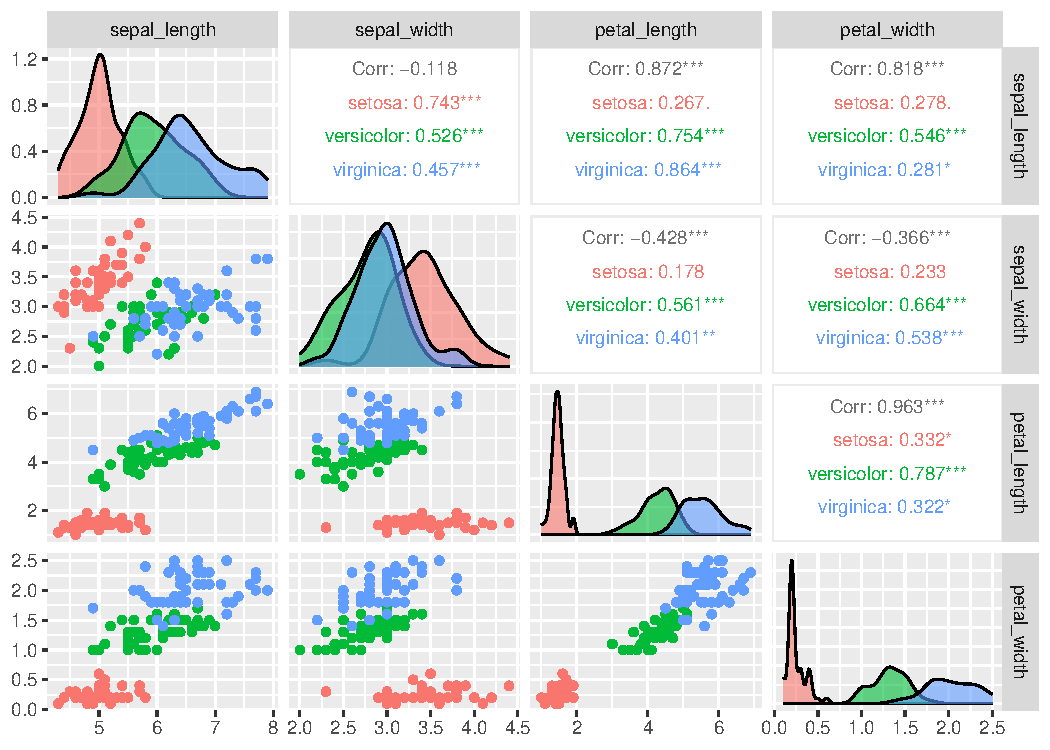
\includegraphics[keepaspectratio]{Análisis-exploratorio_files/figure-pdf/ggpairs-1.pdf}}

}

\caption{Matriz de dispersión y correlación de las variables
cuantitativas (Pearson).}

\end{figure}%

Dado que no se cumple normalidad, también se empleó el método de
Spearman para estimar las correlaciones.

\begin{Shaded}
\begin{Highlighting}[numbers=left,,]
\CommentTok{\# Correlación no paramétrica (Spearman en ggpairs)}
\NormalTok{Fig2 }\OtherTok{\textless{}{-}} \FunctionTok{ggpairs}\NormalTok{(}
\NormalTok{  df,}
  \AttributeTok{columns =} \DecValTok{1}\SpecialCharTok{:}\DecValTok{4}\NormalTok{,}
  \AttributeTok{mapping =} \FunctionTok{aes}\NormalTok{(}\AttributeTok{color =}\NormalTok{ species),}
  \AttributeTok{upper =} \FunctionTok{list}\NormalTok{(}\AttributeTok{continuous =} \FunctionTok{wrap}\NormalTok{(}\StringTok{"cor"}\NormalTok{, }\AttributeTok{method =} \StringTok{"spearman"}\NormalTok{, }\AttributeTok{size =} \DecValTok{3}\NormalTok{)),}
  \AttributeTok{diag =} \FunctionTok{list}\NormalTok{(}\AttributeTok{continuous =} \FunctionTok{wrap}\NormalTok{(}\StringTok{"densityDiag"}\NormalTok{, }\AttributeTok{alpha =} \FloatTok{0.6}\NormalTok{))}
\NormalTok{)}
\NormalTok{Fig2}
\end{Highlighting}
\end{Shaded}

\begin{figure}[H]

{\centering \pandocbounded{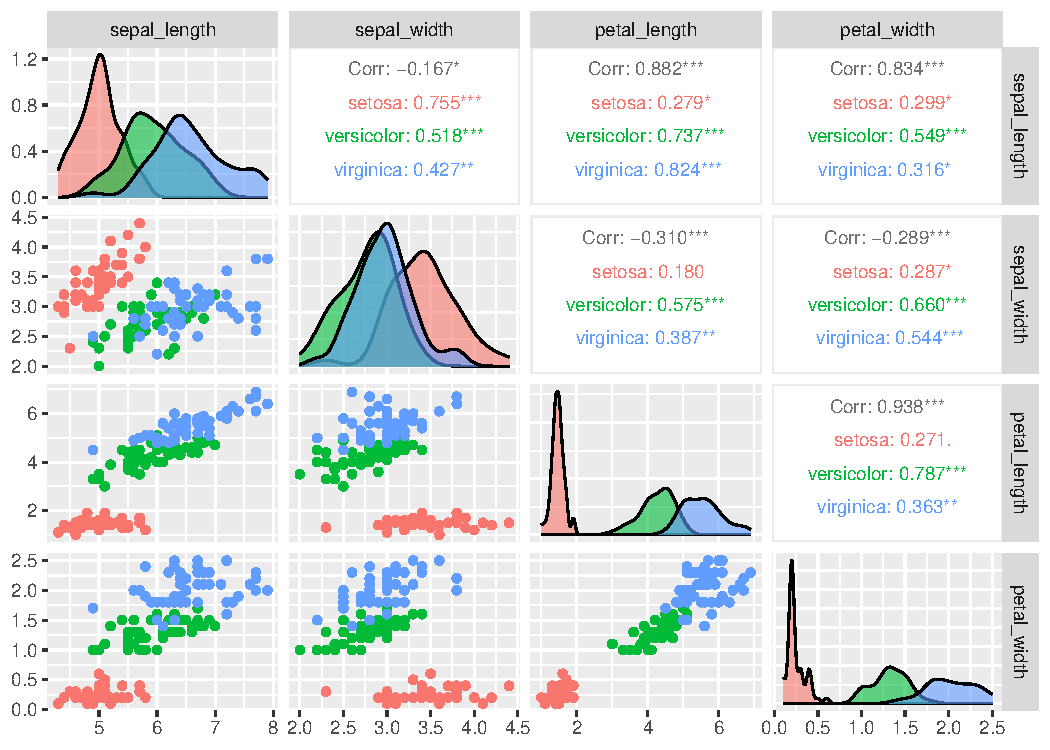
\includegraphics[keepaspectratio]{Análisis-exploratorio_files/figure-pdf/ggpairs 2-1.pdf}}

}

\caption{Matriz de dispersión y correlación de las variables
cuantitativas (Spearman).}

\end{figure}%

\subsection{Distribuciones
univariadas}\label{distribuciones-univariadas}

\begin{itemize}
\item
  \textbf{Sepal.Length:}

  \begin{itemize}
  \tightlist
  \item
    \emph{Setosa} concentrada en valores bajos (4.3--5.8 cm), muy
    homogénea.\\
  \item
    \emph{Versicolor} rango intermedio (≈ 4.9--7.0 cm).\\
  \item
    \emph{Virginica} valores altos (≈ 4.9--7.9 cm), con ligera
    superposición con Versicolor.
  \end{itemize}

  \textbf{Interpretación:} útil para separar Setosa, pero Versicolor y
  Virginica se solapan.
\item
  \textbf{Sepal.Width:}

  \begin{itemize}
  \tightlist
  \item
    Distribución amplia en todas las especies.\\
  \item
    \emph{Setosa} tiende a valores promedio mayores, pero con
    solapamiento considerable.
  \end{itemize}

  \textbf{Interpretación:} bajo poder discriminante, refleja
  variabilidad natural.
\item
  \textbf{Petal.Length:}

  \begin{itemize}
  \tightlist
  \item
    \emph{Setosa} muy bajos (≈ 1.0--1.9 cm), sin solapamiento con otras
    especies.\\
  \item
    \emph{Versicolor} rango medio (≈ 3.0--5.1 cm).\\
  \item
    \emph{Virginica} altos (≈ 4.5--6.9 cm).
  \end{itemize}

  \textbf{Interpretación:} variable clave, separa Setosa y discrimina
  relativamente bien Versicolor vs Virginica.
\item
  \textbf{Petal.Width:}

  \begin{itemize}
  \tightlist
  \item
    \emph{Setosa} muy bajos (≈ 0.1--0.6 cm).\\
  \item
    \emph{Versicolor} rango medio (≈ 1.0--1.8 cm).\\
  \item
    \emph{Virginica} altos (≈ 1.4--2.5 cm).
  \end{itemize}

  \textbf{Interpretación:} la más robusta para separar las tres
  especies, casi sin solapamiento.
\end{itemize}

\subsection{Relaciones bivariadas}\label{relaciones-bivariadas}

\begin{itemize}
\tightlist
\item
  \textbf{Sepal.Length vs Sepal.Width:} nubes muy mezcladas → baja
  capacidad de discriminación.\\
\item
  \textbf{Sepal.Length vs Petal.Length:} relación positiva moderada;
  Setosa queda aislada por pétalos cortos.\\
\item
  \textbf{Sepal.Length vs Petal.Width:} tendencia positiva clara; ayuda
  a diferenciar más que Sepal.Length solo, aunque con solapamientos.\\
\item
  \textbf{Sepal.Width vs Petal.Length / Petal.Width:} relaciones
  débiles, confirman poco valor discriminante del sépalo.\\
\item
  \textbf{Petal.Length vs Petal.Width:} relación lineal muy fuerte, tres
  grupos claramente separados → la mejor combinación para clasificar
  especies.
\end{itemize}

\subsection{Correlaciones numéricas}\label{correlaciones-numuxe9ricas}

Dado que no se cumple normalidad, se utilizaron correlaciones de
Spearman. Los resultados fueron muy consistentes con Pearson, mostrando
que las conclusiones son robustas:

\begin{itemize}
\tightlist
\item
  \textbf{Petal.Length vs Petal.Width:} ρ ≈ 0.93 (Spearman) / r ≈ 0.96
  (Pearson). Correlación extremadamente alta; variables casi
  redundantes, pero en conjunto definen un espacio morfológico clave.\\
\item
  \textbf{Sepal.Length vs Petal.Length:} ρ ≈ 0.88 / r ≈ 0.87. Relación
  fuerte, ambas reflejan gradiente de tamaño.\\
\item
  \textbf{Sepal.Length vs Petal.Width:} ρ ≈ 0.83 / r ≈ 0.82. Correlación
  alta, consistente con patrón de tamaño floral.\\
\item
  \textbf{Sepal.Width con el resto:} ρ entre -0.1 y -0.3 (similares a
  Pearson). Confirma su escaso poder discriminante.
\end{itemize}

\subsection{Interpretación general}\label{interpretaciuxf3n-general}

\begin{itemize}
\item
  Los \textbf{pétalos} son rasgos reproductivos clave: su longitud y
  anchura diferencian a las especies porque están ligados a la atracción
  de polinizadores.
\item
  Los \textbf{sépalos}, en cambio, son estructuras más plásticas y menos
  específicas, lo que explica su bajo poder discriminante.
\item
  La fuerte correlación entre variables de pétalo refleja que ambas
  describen el mismo fenómeno biológico (tamaño floral), pero su
  combinación refuerza la clasificación.
\end{itemize}

La comparación entre Spearman y Pearson muestra que, aunque el supuesto
de normalidad no se cumple, las correlaciones se mantienen prácticamente
idénticas. Esto da confianza en la robustez del patrón biológico: la
diferenciación entre especies de \emph{Iris} depende más de rasgos
reproductivos (pétalos) que de rasgos de soporte (sépalos).

\section{Distribución de variables morfométricas entre
especies}\label{distribuciuxf3n-de-variables-morfomuxe9tricas-entre-especies}

La \textbf{Figura 3} presenta diagramas de caja y bigotes que resumen la
variación de las cuatro variables morfométricas en las tres especies de
\emph{Iris}. Este análisis complementa al resumen numérico y a la matriz
de relaciones bivariadas, ya que enfatiza tendencias centrales,
dispersión y presencia de datos atípicos.

\begin{Shaded}
\begin{Highlighting}[numbers=left,,]
\CommentTok{\# Pasar el dataset a formato largo}
\NormalTok{iris\_long }\OtherTok{\textless{}{-}}\NormalTok{ df }\SpecialCharTok{\%\textgreater{}\%}
  \FunctionTok{pivot\_longer}\NormalTok{(}\AttributeTok{cols =} \SpecialCharTok{{-}}\NormalTok{species,}
               \AttributeTok{names\_to =} \StringTok{"Variable"}\NormalTok{,}
               \AttributeTok{values\_to =} \StringTok{"Valor"}\NormalTok{)}

\CommentTok{\# Gráfico unificado}
\NormalTok{Fig3 }\OtherTok{\textless{}{-}} \FunctionTok{ggplot}\NormalTok{(iris\_long, }\FunctionTok{aes}\NormalTok{(}\AttributeTok{x =}\NormalTok{ species, }\AttributeTok{y =}\NormalTok{ Valor, }\AttributeTok{fill =}\NormalTok{ species)) }\SpecialCharTok{+}
  \FunctionTok{geom\_boxplot}\NormalTok{(}\AttributeTok{outlier.shape =} \DecValTok{21}\NormalTok{, }\AttributeTok{alpha =} \FloatTok{0.7}\NormalTok{) }\SpecialCharTok{+}
  \FunctionTok{facet\_wrap}\NormalTok{(}\SpecialCharTok{\textasciitilde{}}\NormalTok{ Variable, }\AttributeTok{scales =} \StringTok{"free\_y"}\NormalTok{) }\SpecialCharTok{+}
  \FunctionTok{labs}\NormalTok{(}
    \AttributeTok{title =} \StringTok{"Comparación de variables morfométricas en especies de Iris"}\NormalTok{,}
    \AttributeTok{x =} \StringTok{"Especies"}\NormalTok{,}
    \AttributeTok{y =} \StringTok{"Valor (cm)"}
\NormalTok{  ) }\SpecialCharTok{+}
  \FunctionTok{theme\_minimal}\NormalTok{(}\AttributeTok{base\_size =} \DecValTok{13}\NormalTok{) }\SpecialCharTok{+}
  \FunctionTok{theme}\NormalTok{(}
    \AttributeTok{plot.title =} \FunctionTok{element\_text}\NormalTok{(}\AttributeTok{hjust =} \FloatTok{0.5}\NormalTok{, }\AttributeTok{face =} \StringTok{"bold"}\NormalTok{),}
    \AttributeTok{legend.position =} \StringTok{"none"}\NormalTok{,}
    \AttributeTok{strip.text =} \FunctionTok{element\_text}\NormalTok{(}\AttributeTok{face =} \StringTok{"bold"}\NormalTok{)}
\NormalTok{  )}
\NormalTok{Fig3}
\end{Highlighting}
\end{Shaded}

\begin{figure}[H]

{\centering \pandocbounded{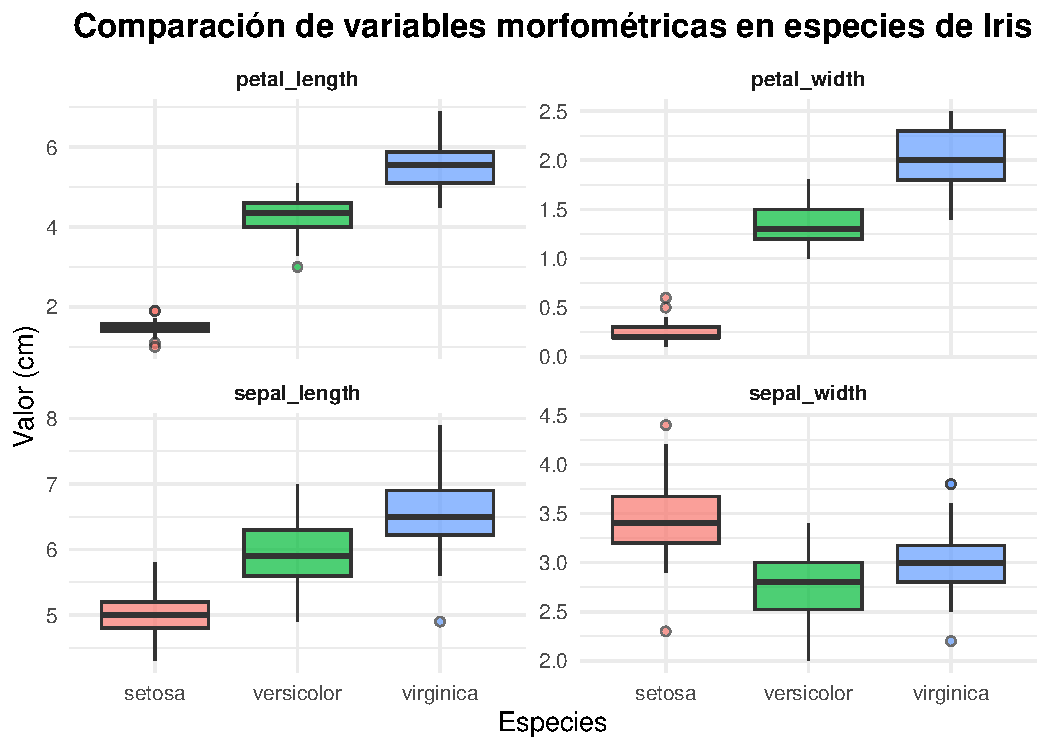
\includegraphics[keepaspectratio]{Análisis-exploratorio_files/figure-pdf/caja y bigotes-1.pdf}}

}

\caption{Distribución de variables morfométricas en tres especies de
Iris.}

\end{figure}%

\subsection{Sepal.Length (longitud del
sépalo)}\label{sepal.length-longitud-del-suxe9palo}

\begin{itemize}
\tightlist
\item
  \emph{I. setosa} muestra valores concentrados entre \textbf{4.3 y 5.8
  cm}, con una mediana cercana a \textbf{5.0 cm}. La caja es compacta,
  indicando baja variabilidad.\\
\item
  \emph{I. versicolor} se distribuye entre \textbf{4.9 y 7.0 cm}, con
  mediana ≈ \textbf{5.9 cm}, rango intermedio.\\
\item
  \emph{I. virginica} alcanza los valores más altos (\textbf{4.9--7.9
  cm}), con mediana ≈ \textbf{6.5 cm}.
\end{itemize}

\textbf{Interpretación}: hay cierto solapamiento entre \emph{versicolor}
y \emph{virginica}. Útil para distinguir a \emph{setosa}, pero no para
discriminar con precisión entre \emph{versicolor} y \emph{virginica}.

\subsection{Sepal.Width (anchura del
sépalo)}\label{sepal.width-anchura-del-suxe9palo}

\begin{itemize}
\item
  \emph{I. setosa} tiene la mediana más alta (≈ \textbf{3.4 cm}), con
  valores entre \textbf{2.3 y 4.4 cm}.
\item
  \emph{I. versicolor} oscila entre \textbf{2.0 y 3.4 cm}, mediana ≈
  \textbf{2.8 cm}.
\item
  \emph{I. virginica} se ubica entre \textbf{2.2 y 3.8 cm}, mediana ≈
  \textbf{3.0 cm}.
\end{itemize}

Se observan varios outliers tanto en \emph{setosa} como
\emph{virginica,} individuos con sépalos inusualmente estrechos. Estos
valores atípicos podrían reflejar variación intraespecífica natural o
condiciones ambientales particulares. La fuerte dispersión y el
solapamiento reducen el valor discriminante de esta variable.

\textbf{Interpretación}: aunque setosa tiende a mayor anchura, la amplia
dispersión y solapamiento hacen que esta variable tenga bajo poder
discriminante.

\subsection{Petal.Length (longitud del
pétalo)}\label{petal.length-longitud-del-puxe9talo}

\begin{itemize}
\tightlist
\item
  \emph{I. setosa} presenta valores muy bajos (\textbf{1.0--1.9 cm}) con
  mediana ≈ \textbf{1.5 cm}.\\
\item
  \emph{I. versicolor} ocupa un rango intermedio (\textbf{3.0--5.1 cm}),
  con mediana ≈ \textbf{4.3 cm}.\\
\item
  \emph{I. virginica} concentra los valores más altos (\textbf{4.5--6.9
  cm}), mediana ≈ \textbf{5.5 cm}.
\end{itemize}

\textbf{Interpretación}: el solapamiento entre \emph{versicolor} y
\emph{virginica} es reducido y se da en los límites
superiores/inferiores de sus cajas. Esta variable es altamente
informativa; separa completamente a \emph{setosa} y discrimina en gran
medida a \emph{versicolor} y \emph{virginica}.

\subsection{Petal.Width (anchura del
pétalo)}\label{petal.width-anchura-del-puxe9talo}

\begin{itemize}
\tightlist
\item
  \emph{I. setosa} tiene los valores más bajos (\textbf{0.1--0.6 cm}),
  con mediana ≈ \textbf{0.2 cm}, sin solapamiento con las otras
  especies.\\
\item
  \emph{I. versicolor} se concentra entre \textbf{1.0 y 1.8 cm}, mediana
  ≈ \textbf{1.3 cm}.\\
\item
  \emph{I. virginica} presenta los valores más altos (\textbf{1.4--2.5
  cm}), mediana ≈ \textbf{2.0 cm}.
\end{itemize}

\textbf{Interpretación}: junto con \emph{Petal.Length}, constituye la
variable más robusta para separar especies; su poder discriminante es
muy alto y con solapamiento mínimo.

\subsection{Interpretación general}\label{interpretaciuxf3n-general-1}

Las variables de pétalo muestran diferencias netas entre especies, con
cajas bien separadas. Por lo que se considera un rasgo clave para
clasificación, debido a su alta capacidad de separar grupos. A
diferencias de las variables de sépalo que presentan mayor dispersión y
solapamiento, lo que limita su valor clasificatorio, debido a su menor
capacidad diagnóstica, más influenciados por plasticidad ambiental.

\section{Análisis de supuestos}\label{anuxe1lisis-de-supuestos}

Se realizó una evaluación de los supuestos básicos, como normalidad,
homocedasticidad y detección de datos atípicos.

\subsection{Normalidad (univariada y
multivariada)}\label{normalidad-univariada-y-multivariada}

\begin{Shaded}
\begin{Highlighting}[numbers=left,,]
\CommentTok{\# Normalidad (univariada y multivariada)}
\NormalTok{mvn\_norm }\OtherTok{\textless{}{-}} \FunctionTok{mvn}\NormalTok{(df[,}\DecValTok{1}\SpecialCharTok{:}\DecValTok{4}\NormalTok{], }\AttributeTok{mvn\_test =} \StringTok{"hz"}\NormalTok{)}

\CommentTok{\# Resultados}
\NormalTok{mvn\_norm}\SpecialCharTok{$}\NormalTok{univariate\_normality}
\end{Highlighting}
\end{Shaded}

\begin{verbatim}
              Test     Variable Statistic p.value    Normality
1 Anderson-Darling sepal_length     0.889   0.023 ✗ Not normal
2 Anderson-Darling  sepal_width     0.908    0.02 ✗ Not normal
3 Anderson-Darling petal_length     7.679  <0.001 ✗ Not normal
4 Anderson-Darling  petal_width     5.106  <0.001 ✗ Not normal
\end{verbatim}

\begin{Shaded}
\begin{Highlighting}[numbers=left,,]
\NormalTok{mvn\_norm}\SpecialCharTok{$}\NormalTok{multivariate\_normality}
\end{Highlighting}
\end{Shaded}

\begin{verbatim}
           Test Statistic p.value     Method          MVN
1 Henze-Zirkler     2.336  <0.001 asymptotic ✗ Not normal
\end{verbatim}

La prueba de Henze--Zirkler indicó que las variables en conjunto no
siguen una distribución normal multivariada (\textbf{HZ = 2.336, p
\textless{} 0.001}). A nivel univariado, el test de Anderson--Darling
mostró que ninguna de las cuatro variables es normal:

\begin{itemize}
\item
  \emph{Sepal.Length}: \textbf{p = 0.023}
\item
  \emph{Sepal.Width}: \textbf{p = 0.020}
\item
  \emph{Petal.Length}: \textbf{p \textless{} 0.001}
\item
  \emph{Petal.Width}: \textbf{p \textless{} 0.001}
\end{itemize}

\textbf{Interpretación:} El conjunto de datos no cumple con la
suposición de normalidad, por lo que deben preferirse pruebas no
paramétricas (ej. Kruskal-Wallis en lugar de ANOVA) y coeficientes de
correlación de Spearman en lugar de Pearson.

\subsection{Homocedasticidad}\label{homocedasticidad}

\begin{Shaded}
\begin{Highlighting}[numbers=left,,]
\CommentTok{\# Homocedasticidad (igualdad de varianzas por especie)}
\NormalTok{levene\_sepal\_length  }\OtherTok{\textless{}{-}} \FunctionTok{leveneTest}\NormalTok{(sepal\_length }\SpecialCharTok{\textasciitilde{}}\NormalTok{ species, }\AttributeTok{data =}\NormalTok{ df)}
\NormalTok{levene\_sepal\_width   }\OtherTok{\textless{}{-}} \FunctionTok{leveneTest}\NormalTok{(sepal\_width }\SpecialCharTok{\textasciitilde{}}\NormalTok{ species, }\AttributeTok{data =}\NormalTok{ df)}
\NormalTok{levene\_petal\_length  }\OtherTok{\textless{}{-}} \FunctionTok{leveneTest}\NormalTok{(petal\_length }\SpecialCharTok{\textasciitilde{}}\NormalTok{ species, }\AttributeTok{data =}\NormalTok{ df)}
\NormalTok{levene\_petal\_width   }\OtherTok{\textless{}{-}} \FunctionTok{leveneTest}\NormalTok{(petal\_width }\SpecialCharTok{\textasciitilde{}}\NormalTok{ species, }\AttributeTok{data =}\NormalTok{ df)}

\CommentTok{\# Resultados}
\NormalTok{levene\_sepal\_length}
\end{Highlighting}
\end{Shaded}

\begin{verbatim}
Levene's Test for Homogeneity of Variance (center = median)
       Df F value   Pr(>F)   
group   2  6.3527 0.002259 **
      147                    
---
Signif. codes:  0 '***' 0.001 '**' 0.01 '*' 0.05 '.' 0.1 ' ' 1
\end{verbatim}

\begin{Shaded}
\begin{Highlighting}[numbers=left,,]
\NormalTok{levene\_sepal\_width}
\end{Highlighting}
\end{Shaded}

\begin{verbatim}
Levene's Test for Homogeneity of Variance (center = median)
       Df F value Pr(>F)
group   2  0.5902 0.5555
      147               
\end{verbatim}

\begin{Shaded}
\begin{Highlighting}[numbers=left,,]
\NormalTok{levene\_petal\_length }
\end{Highlighting}
\end{Shaded}

\begin{verbatim}
Levene's Test for Homogeneity of Variance (center = median)
       Df F value    Pr(>F)    
group   2   19.48 3.129e-08 ***
      147                      
---
Signif. codes:  0 '***' 0.001 '**' 0.01 '*' 0.05 '.' 0.1 ' ' 1
\end{verbatim}

\begin{Shaded}
\begin{Highlighting}[numbers=left,,]
\NormalTok{levene\_petal\_width}
\end{Highlighting}
\end{Shaded}

\begin{verbatim}
Levene's Test for Homogeneity of Variance (center = median)
       Df F value    Pr(>F)    
group   2  19.892 2.261e-08 ***
      147                      
---
Signif. codes:  0 '***' 0.001 '**' 0.01 '*' 0.05 '.' 0.1 ' ' 1
\end{verbatim}

El test de Levene mostró resultados mixtos:

\begin{itemize}
\item
  \emph{Sepal.Length}: \textbf{p = 0.002} → varianzas heterogéneas.
\item
  \emph{Sepal.Width}: \textbf{p = 0.556} → varianzas homogéneas.
\item
  \emph{Petal.Length}: \textbf{p \textless{} 0.001} → varianzas
  heterogéneas.
\item
  \emph{Petal.Width}: \textbf{p \textless{} 0.001} → varianzas
  heterogéneas.
\end{itemize}

\textbf{Interpretación:} Solo Sepal.Width cumple homogeneidad de
varianzas. Las demás variables presentan heterocedasticidad, lo cual
refuerza la necesidad de usar pruebas no paramétricas para comparar
grupos.

\subsection{Outliers multivariados}\label{outliers-multivariados}

\begin{Shaded}
\begin{Highlighting}[numbers=left,,]
\CommentTok{\# Outliers multivariados (Mahalanobis global y robusto)}
\NormalTok{X }\OtherTok{\textless{}{-}}\NormalTok{ df[,}\DecValTok{1}\SpecialCharTok{:}\DecValTok{4}\NormalTok{]}

\NormalTok{center\_global }\OtherTok{\textless{}{-}} \FunctionTok{colMeans}\NormalTok{(X)}
\NormalTok{cov\_global }\OtherTok{\textless{}{-}} \FunctionTok{cov}\NormalTok{(X)}
\NormalTok{d2\_global }\OtherTok{\textless{}{-}} \FunctionTok{mahalanobis}\NormalTok{(X, center\_global, cov\_global)}
\NormalTok{threshold\_global }\OtherTok{\textless{}{-}} \FunctionTok{qchisq}\NormalTok{(}\FloatTok{0.975}\NormalTok{, }\AttributeTok{df =} \FunctionTok{ncol}\NormalTok{(X))}

\NormalTok{mcd }\OtherTok{\textless{}{-}} \FunctionTok{covMcd}\NormalTok{(X) }\CommentTok{\# robusto}
\NormalTok{d2\_robust }\OtherTok{\textless{}{-}} \FunctionTok{mahalanobis}\NormalTok{(X, }\AttributeTok{center =}\NormalTok{ mcd}\SpecialCharTok{$}\NormalTok{center, }\AttributeTok{cov =}\NormalTok{ mcd}\SpecialCharTok{$}\NormalTok{cov)}
\NormalTok{threshold\_robust }\OtherTok{\textless{}{-}} \FunctionTok{qchisq}\NormalTok{(}\FloatTok{0.975}\NormalTok{, }\AttributeTok{df =} \FunctionTok{ncol}\NormalTok{(X))}

\NormalTok{df\_out }\OtherTok{\textless{}{-}}\NormalTok{ df }\SpecialCharTok{\%\textgreater{}\%}
  \FunctionTok{mutate}\NormalTok{(}
    \AttributeTok{d2\_global =}\NormalTok{ d2\_global,}
    \AttributeTok{is\_out\_global =}\NormalTok{ d2\_global }\SpecialCharTok{\textgreater{}}\NormalTok{ threshold\_global,}
    \AttributeTok{d2\_robust =}\NormalTok{ d2\_robust,}
    \AttributeTok{is\_out\_robust =}\NormalTok{ d2\_robust }\SpecialCharTok{\textgreater{}}\NormalTok{ threshold\_robust}
\NormalTok{  )}

\FunctionTok{table}\NormalTok{(df\_out}\SpecialCharTok{$}\NormalTok{is\_out\_global)}
\end{Highlighting}
\end{Shaded}

\begin{verbatim}

FALSE  TRUE 
  144     6 
\end{verbatim}

\begin{Shaded}
\begin{Highlighting}[numbers=left,,]
\FunctionTok{table}\NormalTok{(df\_out}\SpecialCharTok{$}\NormalTok{is\_out\_robust)}
\end{Highlighting}
\end{Shaded}

\begin{verbatim}

FALSE  TRUE 
   95    55 
\end{verbatim}

Se evaluaron outliers multivariados con la distancia de Mahalanobis:

\begin{itemize}
\tightlist
\item
  \textbf{Mahalanobis global (media/covarianza clásica):} detectó
  \textbf{6 observaciones atípicas} de 150 (4\%).\\
\item
  \textbf{Mahalanobis robusto (MCD):} detectó \textbf{55 observaciones
  atípicas} (37\%).
\end{itemize}

\textbf{Interpretación:} El método robusto es más estricto y revela que
una parte considerable de las observaciones no se ajusta al patrón
multivariado esperado. Esto indica que el dataset, aunque muy usado como
ejemplo didáctico, presenta estructuras internas de alta variabilidad
(particularmente en Versicolor y Virginica), lo cual podría influir en
análisis sensibles a outliers (ej. PCA, discriminante).\\
En un reporte real, se recomienda analizar los outliers para verificar
si corresponden a errores de medición, variabilidad biológica genuina o
presencia de subgrupos dentro de las especies.

\subsection{Interpretación general}\label{interpretaciuxf3n-general-2}

Los supuestos paramétricos clásicos (normalidad y homocedasticidad) no
se cumplen plenamente en este conjunto de datos. Por ello, se optó por:

\begin{itemize}
\item
  Usar correlaciones de Spearman en lugar de Pearson.
\item
  Considerar técnicas robustas o no paramétricas en análisis
  comparativos posteriores.
\item
  Los outliers no deben eliminarse automáticamente, sino interpretarse
  en su contexto biológico/ecológico (p.~ej. plasticidad intraespecífica
  en Iris).
\end{itemize}




\end{document}
